\documentclass[]{IEEEtran}
% some very useful LaTeX packages include:
%\usepackage{cite}      
\usepackage{graphicx}   
\usepackage{subfigure} 
\usepackage{url}       
\usepackage{amsmath}    
\usepackage{caption2}
% Your document starts here!
\begin{document}

% Define document title and author
	\title{Weekly Report}
	\author{Adviser: Prof. Yang Wen \\Student: Cheng Wensheng\\ Period: 2018.4.20-4.27
	}
	\markboth{Visual Information Processing Group}{}
	\maketitle

% Write abstract here
\begin{abstract}
	This week I mainly put my effort on making power point slides of CETC 54 and having a meeting on this project.
\end{abstract}

% Each section begins with a \section{title} command
\section{Powerpoint slides}
	% \PARstart{}{} creates a tall first letter for this first paragraph
	\PARstart{A}{fter} reading most classic CNN-based semantic segmentation frameworks, I made a PPT to introduce our research.
	\begin{itemize}
		\item Fully convolutional network set up the foundation for CNN-based end-to-end framework. Its main contribution is to replace the fully connected layers with convolutional layers, which makes it possible to train end-to-end CNN-based frameworks with high precision.
		\item Following works including SegNet, DeepLab, PSPNet, etc. In summary, frameworks can be divided into two parts, i.e., encoder and decoder. Encoder part is used to capture semantic information from shallow to deep, which can be viewed as downsampling. Decoder part can acquire accurate location information, which in nature is upsampling.  Fig.~\ref{fig:mp} is the DeepLab V3 architecture. Fig.~\ref{fig:ss} is the DeepLab V3+ Encoder-decoder architecture.
	\end{itemize}

% Main Part
\section{project meeting}
	% LaTeX takes complete care of your document layout ...
	We took part in the project meeting and discussed some details about the applied project.
	\begin{itemize}
		\item The major point is data. After the meeting, we know that we need to prepare training data by ourselves. The training data only contains R, G, B channels. Besides, we are supposed to get data with multiple resolutions, and find the best corresponding resolution to classify every object. It will take much effort.
		\item About the software framework, although TensorFlow is more mature on Windows, it's better not limit the framework to TensorFlow. Since Pytorch is much easier to create new frameworks and is preferred in research.
	\end{itemize}
\newpage
\begin{figure}[!hbt]
%		 Center the figure.
		\vspace{2cm}
%		\hspace{50cm}
		\begin{center}
			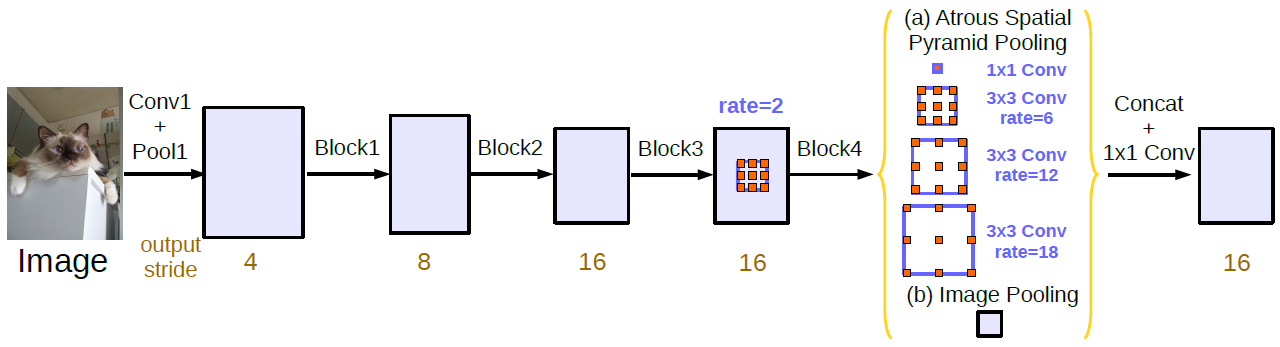
\includegraphics[width=\columnwidth]{dl3}
				%		 Create a subtitle for the figure.
			\caption{DeepLab V3 architecture}
			\label{fig:mp}
		    \hspace{0.5cm}
			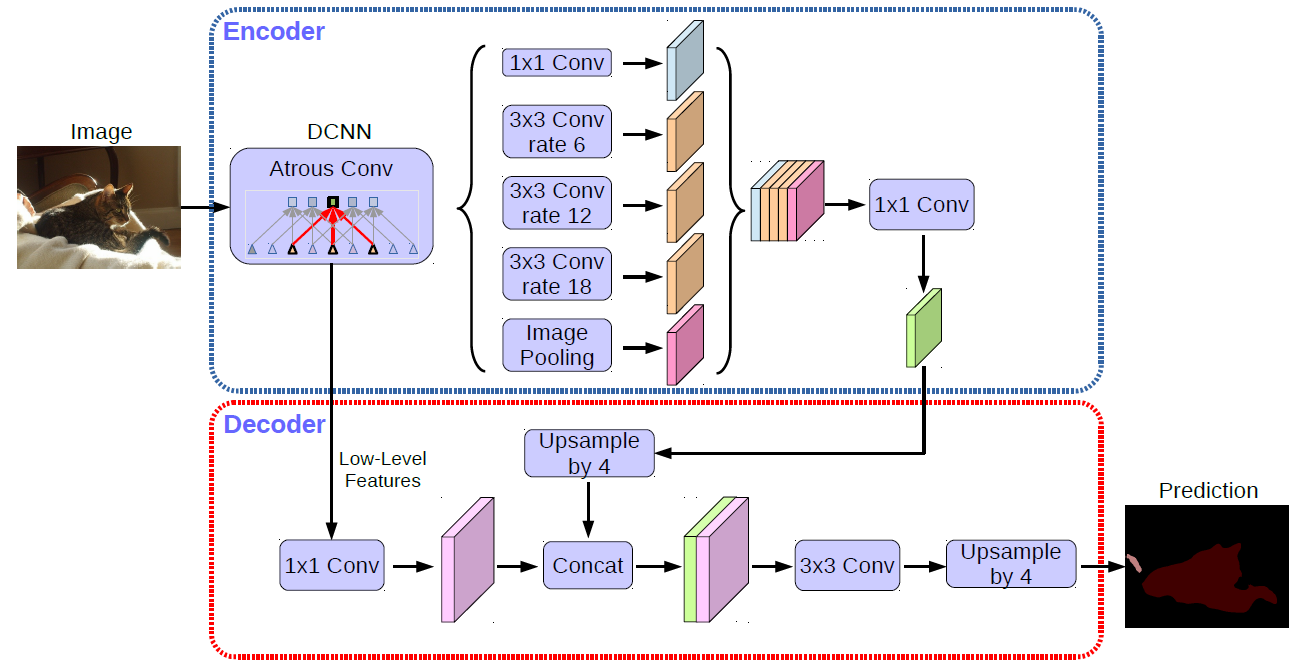
\includegraphics[width=\columnwidth]{dl3pl}
				%Create a subtitle for the figure.
			\caption{DeepLab V3+ Encoder-decoder architecture}
			\label{fig:ss}
		\end{center}
	\end{figure}

% Now we need a bibliography:
%\begin{thebibliography}{5}
%
%	%Each item starts with a \bibitem{reference} command and the details thereafter.
%	\bibitem{HOP96} % Transaction paper
%	J.~Hagenauer, E.~Offer, and L.~Papke. Iterative decoding of binary block
%	and convolutional codes. {\em IEEE Trans. Inform. Theory},
%	vol.~42, no.~2, pp.~429–-445, Mar. 1996.
%
%	\bibitem{MJH06} % Conference paper
%	T.~Mayer, H.~Jenkac, and J.~Hagenauer. Turbo base-station cooperation for intercell interference cancellation. {\em IEEE Int. Conf. Commun. (ICC)}, Istanbul, Turkey, pp.~356--361, June 2006.
%
%	\bibitem{Proakis} % Book
%	J.~G.~Proakis. {\em Digital Communications}. McGraw-Hill Book Co.,
%	New York, USA, 3rd edition, 1995.
%
%	\bibitem{talk} % Web document
%	F.~R.~Kschischang. Giving a talk: Guidelines for the Preparation and Presentation of Technical Seminars.
%	\url{http://www.comm.toronto.edu/frank/guide/guide.pdf}.
%
%	\bibitem{5}
%	IEEE Transactions \LaTeX and Microsoft Word Style Files.
%	\url{http://www.ieee.org/web/publications/authors/transjnl/index.html}
%
%\end{thebibliography}

% Your document ends here!
\end{document}